
%(BEGIN_QUESTION)
% Copyright 2009, Tony R. Kuphaldt, released under the Creative Commons Attribution License (v 1.0)
% This means you may do almost anything with this work of mine, so long as you give me proper credit

Suppose a {\it decade box} resistance unit is used to simulate an RTD signal into a temperature transmitter as such:

$$\includegraphics[width=15.5cm]{i04002x01.eps}$$

Calculate the amount of resistance this decade box would have to be set to in order to simulate the following RTD temperatures:

\begin{itemize}
\item{} Simulate 84 $^{o}$F ; resistance = \underbar{\hskip 50pt}
\vskip 10pt
\item{} Simulate 195 $^{o}$F ; resistance = \underbar{\hskip 50pt}
\vskip 10pt
\item{} Simulate 357 $^{o}$F ; resistance = \underbar{\hskip 50pt}
\end{itemize}

Assume a 100 ohm platinum ($\alpha$ = 0.00385 $\Omega$/$\Omega$$^{o}$C) RTD configuration for the transmitter.

\vskip 20pt \vbox{\hrule \hbox{\strut \vrule{} {\bf Suggestions for Socratic discussion} \vrule} \hrule}

\begin{itemize}
\item{} Explain why {\it four} wires are being used here for this RTD transmitter calibration.
\item{} If you consult a {\it table} for resistance values of a 100 ohm platinum RTD with an alpha value of 0.00385, you will find the numbers slightly disagree with those predicted by the equation.  Explain why.
\item{} Students very commonly mis-interpret the symbols drawn next to the input terminals of an RTD transmitter, especially the terminals which must be made common to each other at the sensor.  One of the most popular misconceptions  is to think that those terminals shown common to each other by the symbol are already joined together {\it inside the transmitter}.  Explain why this interpretation cannot be true, based on how you know 3-wire and 4-wire RTD circuits are designed to work.
\end{itemize}

\underbar{file i04002}
%(END_QUESTION)





%(BEGIN_ANSWER)

\noindent
{\bf Partial answer:}

\vskip 10pt

\item{} Simulate 357 $^{o}$F ; resistance = \underbar{169.51 $\Omega$ (calculated)} \hskip 10pt \underbar{168.68 $\Omega$ (according to table)} 

%(END_ANSWER)





%(BEGIN_NOTES)

\begin{itemize}
\item{} Simulate 84 $^{o}$F ; resistance = \underbar{111.12 $\Omega$ (calculated)} \hskip 10pt \underbar{111.24 $\Omega$ (according to table)}
\vskip 10pt
\item{} Simulate 195 $^{o}$F ; resistance = \underbar{134.86 $\Omega$ (calculated)} \hskip 10pt \underbar{134.92 $\Omega$ (according to table)}
\vskip 10pt
\item{} Simulate 357 $^{o}$F ; resistance = \underbar{169.51 $\Omega$ (calculated)} \hskip 10pt \underbar{168.68 $\Omega$ (according to table)} 
\end{itemize}

\vfil \eject

\noindent
{\bf Summary Quiz:}

Calculate the temperature of a platinum RTD with an alpha of 0.00392 and a measured resistance of 173.9 ohms.

\begin{itemize}
\item{} 68.17 $^{o}$C 
\vskip 5pt 
\item{} 188.5 $^{o}$C
\vskip 5pt 
\item{} 443.6 $^{o}$C
\vskip 5pt 
\item{} 206.0 $^{o}$C 
\vskip 5pt 
\item{} 191.9 $^{o}$C 
\vskip 5pt 
\item{} 202.3 $^{o}$C 
\end{itemize}

%INDEX% Measurement, temperature: RTD resistance calibration

%(END_NOTES)


